\documentclass{book}
%\documentclass{scrartcl}
% borrowed from the patterns book ~/oldHome/writing/patterns/book.tex

%\paperheight=9.5in
%\paperwidth=6.5in
%\pdfpageheight=9.5in
%\pdfpagewidth=6.5in

\usepackage{graphicx}
\usepackage{makeidx}
\usepackage{footnote}
\usepackage{appendix}
\makeindex

% goto http://web.image.ufl.edu/help/latex/latex_indexes.shtml
% to read about index creation
% summary:
% simple\index{simple}
% deeper\index{under!something!else}
% see\index{example|see{simple}}

\textheight     7in
\textwidth      4in
%\textheight     9in
%\textwidth      6.75in
\topmargin      -0.5in
\oddsidemargin  0.1in
\evensidemargin -0.1in
\setcounter{tocdepth}{1}
\setcounter{secnumdepth}{3}

\begin{document}
\frontmatter
\pagestyle{empty}
\pagenumbering{roman}
\title{A Very Introductory Compilers Course}
\author{Phil Crow}
\date{}
\maketitle

\noindent
\textbf{Compilers} \\
A Very Introductory Compilers Course \\
by Phil Crow \\

\vspace{.2in}
\noindent
Copyright \copyright 2023 Phil Crow (crow.phil at gmail.com).

\noindent
This work is covered by two licenses.  First, you may use the code examples
under the same terms as Perl 5.36.1 or the terms of any later version
of Perl at your option.

Second, the text is licensed under the
Attribution-Noncommercial-Share Alike 3.0 United States License
from Creative Commons.
To view a copy of this license (and a summary of its terms), visit

\begin{verbatim}
http://creativecommons.org/licenses/by-nc-sa/3.0/us/
\end{verbatim}

Everything is on github\footnote{https://github.com/philcrow/compilerclass/tree/main/book} where I am philcrow.

\newpage
\pagestyle{headings}

\begin{center}
\textit{For Dad, who was always curious.}
\end{center}

\tableofcontents

\chapter*{Preface}

There are usually two sides to technology: using it and working on it.
Loosely, I call this driver's ed vs. auto shop. In the former we learn
to operate a car: parking, signaling, turning, minding the rules of the
road. In the latter we would learn to repair the various systems on
a car. Notice I say ``would learn.'' I've never taken auto shop. My
repair skills are limited. This is typical. More people need to know
how to operate a car than need to know how to work on one.

For the expert, shop is more interesting. The temptation to fixate on it
is strong. This definitely holds for books and courses about compilers.
This book takes the driver's ed approach exclusively. It is completely
distinterested in how finite automata and context free grammars work
theoretically and how they are implemented. Our goal will be to use
tools to make languages.

One of the important inovations in software development since the start
of my career has nothing to do with code. It is the
agile process. One of the key concepts of agile development is the Minimum
Viable Product (MVP). The idea is to build something that will run and
deliver some value to the users. After it is in the users' hands, revisit
the product to add features. That will be my approach here.

We will start with the smallest language I could conceive. It will only add
single digit integers. When it does so, it will only print the
result to standard out. Then we will commence adding features to this
language. How far you take it is up to you. At least we want variables,
flow of control (conditional logic and some sort of loop), plus
functions which return values which can be called recursively.
We could go on to add types and type checking, arrays, and many other
features. Remember the goal: to learn the tools of language construction
and play with the language feature trade offs. If you are a student,
when you complete this work, you should be able to imagine implementing
a domain specific language or code generator. You will also learn
the basic concepts in case you have an interest in working on production
compilers (the auto shop part).

The main tool of this course is ANTLR4 which was written by Terence Parr.
He wrote an excellent book about it called
{\it The Definitive ANTLR4 Reference}.
You will probably want to consult that, or the various forms of online
documentation including especially antlr.org. I will shamelessly begin
by implementing the language for arithmetic he lays out there. Extensions
and poor choices are mine alone.

You can use ANTLR4 with various languages including C, C\verb+#+, JavaScript,
and Python. Here I use Python. It is cleaner to look at than some
other languages. If you are going to follow along, choose a language
that is comfortable for you. Follow the insructions to obtain the
run time for your chosen language at antlr.org.

Let's get started.


\mainmatter
\pagenumbering{arabic}

\part{A Simple Compile and Go Language}

\chapter{Getting Started}

There are two parts to beginning work on compilers. One is understanding
the goal. The other is installing the tools. This chapter takes those in order.

\section{What are Trying to Do?}

Compiling is translating a human readable source code language
into something else called the target language. I'm going to give
meaning to that one sentence definition with a series of examples.
These are live programs you can install from the internet that
perform some kind of compilation. All of these run well at a
unix command line. If you have a Mac or Linux system, open a terminal
window. If you have a Microsoft Windows system use powershell.

\subsection{gcc}

Traditionally, the target language is assembly. The most famous
current compiler following this tradition is gcc. Given a C program,
it will generate assembly, then quietly assemble and link that, so you
receive an executable. How portable will the executable be? Not very.

{\footnotesize
\begin{verbatim}
    #include <stdio.h>

    int main(int argc, char *argv[]) {
        printf("Hello %s\n", "Rob");
        return 12;
    }
\end{verbatim}
}

Compile and run:

{\footnotesize
\begin{verbatim}
    gcc hello.c -o hello
    ./hello
    echo $? # to see the exit status
\end{verbatim}
}


From the gcc website\footnote{https://gcc.gnu.org/}
you can see that gcc is actually more than a c compiler.
That's just its most famous feature.

\subsection{dot}

There are lots of other related tools which don't generate assembly,
many of which don't make anything that actually runs. One of my favorites
is Dot\footnote{https://graphviz.org/}. It takes a descriptive source
language and generates image output in formats like png, jpeg, gif,
pdf, and others.

If you install graphviz on your system, you can save this as family.dot
in your favorite text editor:

{\footnotesize
\begin{verbatim}
    digraph { Mom -> Me }
\end{verbatim}
}

Compile it, with this command:

{\footnotesize
\begin{verbatim}
    dot -Tpng -o family.png family.dot
\end{verbatim}
}

Then you will have png output in family.png showing this tiny excerpt
of my family tree.

You can learn all about dot and its relatives in the graphviz family
at their website\footnote{https://graphviz.org/}.

If you don't want to install graphviz on your system, you can
still play with it on a site like: https://sketchviz.com/new

\subsection{TeX}

TeX is a language for typesetting written by Donal Knuth (who also
wrote a famous set of books on the art of programming). You can write
macros in it. Leslie Lamport wrote a whole bunch of really useful ones
which he called LaTeX. I used LaTeX to make this book. In TeX,
you type commands that describe documents, and the contents of those
documents, into a text editor. Here is an example:

{\footnotesize
\begin{verbatim}
    \documentclass{article}
    \title{A Sample}
    \author{Phil Crow}
    \begin{document}
    \maketitle

    This is a simple sample of a LaTeX article.

    \end{document}
\end{verbatim}
}

Save that as article.tex, to make a PDF run

{\footnotesize
\begin{verbatim}
    pdflatex article.tex
\end{verbatim}
}

This is my preferred mode of PDF generation. There is a vibrant
online community around LaTeX\footnote{https://www.latex-project.org/}.

\subsection{lilypond}

Han-Wen Nienhuys and Jan Nieuwenhuizen thought it would be
cool to use TeX to engrave sheet music. They developed lilypond,
which long ago gave up on using TeX. The syntax still looks a lot
like TeX.

Given a text file called scale.ly with this content:

{\footnotesize
\begin{verbatim}
    \score{
        {
            c' d' e' f' g' a' b' c''
        }
        \layout{}
        \midi{}
    }
    \version "2.18.2"
\end{verbatim}
}

To generate sheet music as a PDF type:

{\footnotesize
\begin{verbatim}
    lilypond scale.ly
\end{verbatim}
}

Since the layout and midi commands are there, you also get scale.midi
with a grand piano playing the music.

As you may have noticed, I am rather obsessed with tools that take
source from a text file and produce something useful.

\subsection{Typescript}

JavaScript is one of my favorite languages. Since the browser takes
care of running it, I can get all kinds of spectacular behaviors
for users with it, often in only a few lines. It also reminds me
of other languages I have enjoyed in the past, like Perl.

There are those who have a dislike for languages like this in general
(loosely typed, being the main complaint). Many different groups of
JavaScript haters have developed alternatives.

One of those is Typescript. You write in Typescript, then convert
it to JavaScript, since that is the only language the browsers understand.

Languages that convert one source language to another are called transpilers.

If you want to play with it see their
website\footnote{https://www.typescriptlang.org/play/}.

You can also install it on your system.

\subsection{Sass}

CSS is the language which controls the appearance of web pages. It is
also often maligned. CSS is descriptive, that is it has no conditionals
or loops. As with JavaScript, many have tried to improve it by making
a super-language which is more expressive, but can be transpiled to CSS.
The one I have heard the most about is Syntactially Awesome Style Sheets
(Sass).

To read more about it see their
website\footnote{https://sass-lang.com/guide}.

\subsection{Virtual Machines}

Returning to languages that run, we find that an executable for the
system where the compiler ran is not the only option. Some languages
target a virtual machine.

In the late 1970s computers were a hot new thing. Size was coming down.
You no longer needed a room (with its own air conditioner) to house one.
The problem was that everyone was building them, each using a different
architecture. Infocom wanted to produce games. The problem was how to
make them run on whatever system the customer bought.

Joel Berez and Marc Blank answered that question by developing a
device indpendent virtual machine called the Z-Machine. For each new
computer that came out, a small number of developers at Infocomm
would port that to the new platform. All the games compiled to its
format. Once the port was finished the whole line of games would
work on the new system.

There were virtual machines before this. And, there is a famous one
that came later called the Java Virtual Machine. The idea is always
the same. Compile the source code to the format of the virtual machine.
Port the virtual machine to all platforms of interest. All the programs
run on all the platforms.

\subsection{Summary}

Compilers take source language from a text file that humans can read
and write. They turn that into another language or format, usually
one that humans would find hard to read, but that the computer can
render or run.

\section{What Tools will we Use?}

Our goal in this course is to implement a small language, or really
a series of small lanuages of increasing utility (and corresponding
complexity). To do this, we will describe out languages with ANTLR4.

To follow along, you need to install (in order) a Java Development
Kit (JDK), gradle, and ANTLR4. You don't have to use these tools.
I have learned a lot about compilers by reading books and translating
their examples from the language in the book to the language I prefer.
You could do the same, but I won't spend time worrying about you then.
Note also that ANTLR4 is written in Java, so installing a JDK is not
optional with it, you can generate lots of other languages like
the currently popular Python.

Visit https://openjdk.org/ if you need to install Java.

Visit https://gradle.org/ if you need to install gradle.

Visit https://www.antlr.org/ to install ANTLR4.

If you want to generate assembly, you need an assembler. Good news:
gcc has that inside it. That's one choice. I also have a little
pseudo-assembler I wrote to give a feel for assembly without worrying
about actual chip instructions.

\chapter{Compilation}

Before we start writing our own language, it is important to understand
how a compiler does its translation work.

All quality software is made in modules. Each module is focused on one
task. The inputs and outputs to it are clearly defined. If we reject
the design of a component, we can replace it. So long as the inputs and
outputs are the same, none of the other modules need alterations. Compilers
are modular.

To deduce what the compiler modules should be, think about the work to
be done. At the beginning there is a source file. We need to read that
text. This reading happens one character at a time, because many
of the things we care about are only one character, like a plus sign.

From the raw stream of characters, the next step forms tokens. These
are the basic elements of a program like a keyword, a brace, a number, or
one of those plus signs. The module that forms the tokens is called
the scanner, the tokenizer, or the lexer. That last term comes from
the longer name of this process: lexical analysis. Always remember
that the tokens are formed first. Nothing that happens further downstream
can adjust how the lexer formed the tokens.\footnote{There are other
parsing schemes where this is not the case, notably recursive descent
parsing favored in Perl and Raku. We won't go into that here.}

Given the token stream, the parser attempts to recognize the language
based on its gramamr. When that works, it builds an abstract syntax
tree (AST) which represents the particular program in a data structure.

With an AST you can immediately interpret the language, which is what we
will mainly do. You can also build a secondary tree (or directed graph).
Such a tree allows you to do two things: (1) further analize the program
for semantic errors, (2) optimize the program, which is usually to make
it run faster and/or use less memory.

Semantic analysis and optimization are optional additional modules in the
chain. You can have several of each. All of those take and produce
the same internal representation. That allows us to mix and match them.

Finally, the last module emits a target language. Notice that this
"finally" might in fact kick off further processing. For instance, if you
make a PDF, you would still need a viewer to render it. Or, in a setup
like gcc, you would emit assembly, then immediately assemble and link
the result into an executable. In that case, assembling and linking would
be additional steps.

This is what the whole process looks like from source to target.

\begin{figure}
\centering
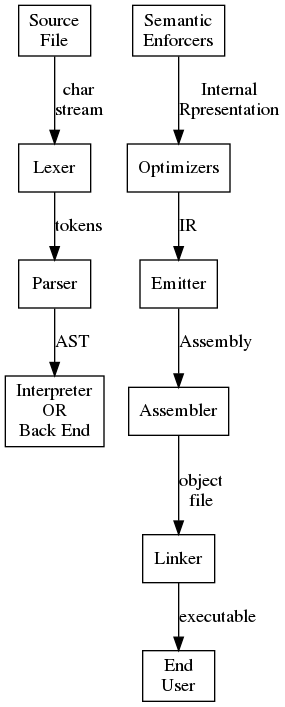
\includegraphics[scale=0.70]{compilationsteps.png}
\end{figure}

I've divided this at a logical point partly for screen layout,
but also to show the front and back halves of the chain.

The parser makes the AST. Something walks that. To start, we will
walk that with an interpreter and avoid the back half entirely.
If you move on to the back, you need the visitor to make an internal
representation (IR). This is either another tree or a directed graph.
That is what the semantic analyzers, optimizers, and emitters use.

Again, after you emit the target language compilation is finished,
but the process might continue. Perhaps you need to bundle the result
into a form that can be delivered economically to a browser, or your
target was assembly that needs to be assebled and linked. We won't
have any concern for those final steps. Once the target is reached,
we will leave the rest of the tools to others.

\include{addingDigits}
\chapter{Regular Expressions}

One of the key failings of our digit adder from the last chapter is that
it only handles one digit numbers. A first improvement was an exercise:
expand to handle more integers. To do this we need to learn a bit about
regular expressions.

\section{Multiplicity}

We often want to allow a matched item to be repeated. Here we want more
digits. In other case we might want multiple statement in a block,
or multiple parameters in a function definition. Regular expressions
provide this. There are three basic operators to help us. We can also
use these in grammar rules.

When we want one or more of something, we use a trailing plus (+). So,

    [0-9]+

is a naive way to solve the single digit problem. Now we can have any
integer.

We don't need the other multiplicities now, but it makes sense to talk
about them together.

Sometimes we want something to be optional, but repeatable. One example
is else if after an if construct. When you use conditional logic, you don't need
any else or else if blocks. But, you can have as many of the latter
as you like. For this we use an asterisk (*). Suppose that we have
already defined what we mean by elseif, using a grammar rule with that name.
Then we can allow zero or more of those with

    elseif*

Finally, sometimes we want something to be optional. That is, we want
zero or one. For that we use a question mark (?). For instance, we could
allow negative numbers with an optional leading minus sign.\footnote{
This is not the ideal way to account for negative numbers. We should use
a unary negation operator instead.}

    '-'? [0-9]+

To summarize

\begin{tabular}{l l}
    Operator &      Meaning \\
    +        &      One or more \\
    \verb+*+ &      Zero or more \\
    ?        &      Optional (zero or one) \\
\end{tabular}

\section{Alternatives}

We can use

    NUMBER: [0-9]+;

to allow multi-digit integers. But, that allows things we probably don't
want, like 00001. In some languages a leading zero forces the number to
be octal. We don't want people to think that is happening in our language.

If we want a more traditional number, we need more than one expression.
We need to be able to pick between expressions. In regular expressions,
we use a pipe symbol (\verb+|+) to indicate choose one of these. This allows us
to have zero and non-zero numbers, but not leading zeros.

{\footnotesize
\begin{verbatim}
    NUMBER: '0' | [1-9] [0-9]* ;
\end{verbatim}
}

This says: A NUMBER is a literal zero OR any digit 1-9 optionally
followed by any digit. Note that the notion of `and' is achieved by
setting two expressions side-by-side, but the order is enforced.

\section{Excercises}

\subsection{Rational Numbers}

In the last chapter I used the python int function to convert our numbers
from strings for calculation. I could have used float instead. Then,
we could use rational numbers instead of integers. This seems like
a good idea. Write a definition of NUMBER which allows for positive
rational numbers. Hint: alternatives are important here and the first
one is zero by itself. Hint 2: consult www.json.org for
a railroad track diagram of number.

\subsection{Variable Names}

Jump ahead in your thinking to imagine our language has variable.
Write a token rule to define them. What symbols will be allowed in
variable names? Can all of those be in the first position?
Note that character classes can any number of ranges, which can
include letters like a-f. They can also include single characters.

\chapter{Arithmetic}

In his book {\it The Definitive ANTLR 4 Reference}, Terence Parr
provides a language for basic arithmetic. I'm going to borrow that
with a few twists.

This version of the language will support addition, subtraction,
multiplication, division, and parentheses for their usual role in
controlling precedence. It will also introduce variables which must
be assigned a value before use, but then can appear anywhere a number
is allowed.

\section{Grammar}

We need to learn quite a few features of ANTLR grammars to expand our
languate in this way. This section details those grammar features.
Later in the chapter we will see how to use the new grammar to perform
arithmetic by implementing a visitor.

\subsection{Arithmetic}

To start, I will present just the arithmetic, leaving variables for
a later section.

I'm going to present the new grammar a bit at a time so we can digest it.
All of this goes in the new Calc.g4.

The first big change is that we need more rules. We want to allow
multiple statements in a program. This requires introducing a rule
for statements and making a program depend on those.

{\footnotesize
\begin{verbatim}
    grammar Calc;

    program: statement+ ;
\end{verbatim}
}

Note that we use the same multiplicity operators for rules as
for regular expressions. So, this reads: ``A program is one or
more statements.''

To start, we will have two types of statements: one for expressions
and one for blank lines. It is not nice to work in a language that
prevents us from having vertical space between sections of interest.
This requires the second new grammar feature: alternatives.

{\footnotesize
\begin{verbatim}
    statement: expression NL
             | NL
             ;
\end{verbatim}
}

The pipe symbol means or (which you might also remember from regular
expressions). This reads as: ``A statement is either an expression
followed by a new line OR a bare new line.''

Note that it is typical to list each alternative on a separate line
and to align the colon and pipes vertically. For extra clarity,
the semi-colon has its own line.

Later we will add a variable assignment statement as an alternative.

Defining what we mean by a statement has introduced two new undefined
terms. This is typical in grammar work. We have to keep defining
until everything has a rule or token definition.

For arithmetic we need the four operations and parentheses. Recall
that precedence matters a lot for this kind of routine Math.

An expression like

{\footnotesize
\begin{verbatim}
    3 + 4 * 5
\end{verbatim}
}

could be computed exclusively left to right. Then, three plus four
is seven, which multiplied by five is 35. But, that isn't what we
would normally do. Instead, multiplication would take precedence.
Thus, as we learned in school, we should multiply four by five to
make twenty, then add three for an answer of 23.

When you design a language, you have full control. It is within your
power to defeat convention. Sometimes that is exactly what you should
do. But, as Larry Wall frequently writes, you should normally abide
by the principle of least surprise. It would be very surprising to
have the rules from school ignored here.

How do we tell ANTLR about our desire for normal precedence?
We list the higher precedence operation first. That is a simple
principle, but it requires some contortion when two or more operations
need to be at the same precedence level, as we are about to see.

{\footnotesize
\begin{verbatim}
    expression: '(' expression ')'
              | expression (STAR|SLASH) expression
              | expression (PLUS|MINUS) expression
              | NUMBER
              ;
\end{verbatim}
}

The first alternative is anything in parentheses.\footnote{This doesn't
actually have to be listed first to win a precedence race. The parenthesis
token is only valid for this rule, so it would win regardless of order.}
Then comes multiplication and division in an alternative together.
They are followed by addition and subtraction in a joint alternative.
At the end is the humble number.

Note that I have chosen to name the operator tokens rather than using
literals. This will make it slightly easier to determine which operation
matched when we have to choose between addition and subtraction or
multiplication and division.

We have our rules. Now it remains to define the tokens.

{\footnotesize
\begin{verbatim}
    NL          : '\r'? '\n' ;
    NUMBER      : [0-9]+ ;
    STAR        : '*' ;
    SLASH       : '/' ;
    PLUS        : '+' ;
    MINUS       : '-' ;
    HS          : [ \t] -> skip ;
\end{verbatim}
}

A newline (NL) is an optional carriage return and a required line feed. This
accounts for the two common line endings. Microsoft Windows uses both
characters. Unix systems, including Macs, use only the line feed.

A NUMBER is still the integer only first thought version from a prior
chapter. If you did the exercise to improve it, use that instead.
Also, consider moving to floats here.

The arithmetic tokens (STAR, SLASH, PLUS, and MINUS) are just names for
the characters.

Finally, HS is horizontal space. This is the answer to an exercise
from a prior chapter. This character class includes spaces and tabs.
The special dash arrow syntax allows us to immediately act within the
lexer. By choosing skip as that action, the spaces we don't care about
a discarded.\footnote{If you need to use spaces, you have to be more
careful. You would need them for a language like python where they matter,
or if you want to emit source code that looks the same as the original,
possibly for error message reporting. Ask the internet what to do in
those cases.}

\subsection{Variables}

To introduce variables, we need only three things: a new statement
alternative for assigning to them, a new expression for using them
in other expressions, and a token controlling their legal name pattern.

{\footnotesize
\begin{verbatim}
    statement: ...
             | ID '=' expression NL
\end{verbatim}
}

An assignment statement is a variable name (ID), a literal equal sign,
any expression, and a newline.

{\footnotesize
\begin{verbatim}
    expression: ...
              | ID
\end{verbatim}
}

Any legal variable name can be used directly in any other expression
as if it were a literal number. Note that that grammar cannot enforce
our rule that a variable needs to have a previous assignment before use.
That is a semantic rule. We will need to enforce that after the parser
builds the abstract syntax tree (AST).

The token for a variable name can be simple.

{\footnotesize
\begin{verbatim}
    ID : [a-z]+ ;
\end{verbatim}
}

This allows any lowercase letters. Most languages are more generous.
Look for an exercise to address this.

\subsection{Labels}

We can use the grammar from the last sections, but it will require
quite a bit of extra work. It would generate a single visitStatement
method and a single visitExpression method. We would need conditional
logic to figure out which rule matched before we could do our computations.

To help us, ANTLR provides labels. They look like comments, but
are requests for extra methods with supplied names. At the end of
each alternative, we add a pound sign (\verb+#+) and the name we want.
I'll show the complete grammar now, notice the labels.

inject Calc.g4 from (stages/arithmetic)

There are two other labels. In the expression
alternatives\footnote{Rule alternatives are sometimes called productions.
That is because in tools like yacc there would be code to make AST nodes
after the match rule. ANTLR is producing those AST nodes for us, so it
is still a production, just an automated one.} for multiplication/division
and addition/subtraction, I labeled the operator match fragment `op`.
That will generate a useful attribute of the context objects with that
name. We'll see that this makes it easier to pick between the two
operations sharing each precedence level.

\section{Visitor Implementation}

Now that we have the grammar, we can generate the lexer, parser, and
visitor base class.

{\footnotesize
\begin{verbatim}
    antlr Calc.g4
\end{verbatim}
}

We need the same three code files as for the single digit adder:
a test, a driver, and the visitor. Since the grammar has the same name,
we can use the driver from the single digit adder without modification.
We can also use the test class, but we will want to expand it to cover
the new language features. Thus, I will only show the new visitor.
You need to write tests to cover every feature of the language.

\subsection{Numbers}

In a visitor, the methods return something useful. In our case that
will be the calculation result for expressions. If we were continuing
compilation with semantic analysis, optimization, and emission, we would
need to return nodes that formed a tree or digraph.

One of the nice features of ANTLR is that you can work in stages.
This fits our minimum viable product/enhancement approach. Start with
the minimum. We need only the visitPrint and visitnNumber to make
the first test pass.

Here is the test class

{\footnotesize
\begin{verbatim}
    class TestVisitor(unittest.TestCase):
        def test_number(self):
            program = "4\n"
            tree = self.get_tree(program)
            visitor = Visitor()
            answer = visitor.visit(tree)
            self.assertEqual(4, answer)

        def get_tree(self, program):
            input_stream = InputStream(program)
            lexer = CalcLexer(input_stream)
            stream = CommonTokenStream(lexer)
            parser = CalcParser(stream)
            tree = parser.program()
            return tree

    if __name__ == '__main__':
        unittest.main()
\end{verbatim}
}

This is similar to the one we saw when testing single digit adding.
But, I have made a helper (\verb+get_tree+) to handle the standard compilation
steps that lead to the AST.

Notice that the program in \verb+test_number+ is just a four and a newline.
We required the newline statement terminator in our grammar. ANTLR
won't recognize the statement without it. When we visit the tree,
we will receive the return value of the visitProgram method. We don't need
to implement that. The inherited one will do nicely.

When the visitor sees our program, it will first capture the number,
then the new line. From the grammar, this will become a tree like
this\footnote{This tree uses the labels for statement and
expression alternatives.}:

{\footnotesize
\begin{verbatim}
    program
       |
     print    
    /     \
   number  NL
     |
   NUMBER
     |
     4
\end{verbatim}
}

Each of the rule alternatives in this tree will have a method in
the generated CalcVisitor. That's why we need to implement visitPrint
and visitNumber.

To make this test pass, we need only visitPrint and visitNumber in
our Visitor.py:

{\footnotesize
\begin{verbatim}
    from CalcVisitor import CalcVisitor
    from CalcParser import CalcParser

    class Visitor(CalcVisitor):
        def visitPrint(self, ctx:CalcParser.PrintContext):
            answer = self.visit(ctx.expr())
            print(answer)
            return answer

        def visitNumber(self, ctx:CalcParser.NumberContext):
            answer = int(ctx.NUMBER().getText())
            return answer
\end{verbatim}
}

This visitNumber shares some features with visitProgram from our single
digit adder. In particular, it invokes NUMBER as a method on the context
object. In this case, there is only one number in the rule alternative,
so there is no argument. Calling getText returns the string that matched.
Python provides the int builtin function to convert that string to an
actual number. If you expand the definition of number to allow
decimals, switch from calling into to calling float.

I collected the answer on one line, then returned it on a separate line.
That allows me to add debugging with the answer as needed.

In visitPrint, I do the actual printing. But, I also return the value
so tests don't have to trap the console output to make their assertions.

\subsection{Operations}

Now that we are handling number expressions, we can move up to
calculating. Let's look at visitAddSubtract.

{\footnotesize
\begin{verbatim}
        def visitAddSubtract(self, ctx:CalcParser.AddSubtractContext):
            left = self.visit(ctx.expression(0))
            right = self.visit(ctx.expression(1))
            if ctx.op.text == '+':
                answer = left + right
            else:
                anwer = left - right
            return answer
\end{verbatim}
}

There are two expressions involved in these
operations\footnote{which is why we call them binary operations}.
If you look in AddSubtractContext in the grammar, you can see that
the expression method takes an argument. As with the single digit
adder, call that with zero and one to get the two operands.
The visit will terminate at either a number or an id expression,
both of their visitors return integers ready for computations.

In the grammar, I labeled the operator `op`. That created an attribute
of the context class with that name. It is an object of type
CommonToken, which has a text attribute. That tells us which symbol
matched. We know we are either adding or subtracting, so we can
test for plus sign. If it is plus, we add, otherwise subtract.

Again, I stored the calculation result in answer, so that I can
add debugging as needed.

I won't show visitMultiplyDivide. You can work that out for yourself.

\subsection{Variables}

There are two visit methods for variables: visitAssign and visitId.
The first one needs to compute the right hand side expression and
store it. The second one needs to look up that answer when it appears
in a subsequent expression. Start with a test

{\footnotesize
\begin{verbatim}
        def test_var(self):
            program = "x=3\nx+4\n"
            tree = self.get_tree(program)
            visitor = Visitor()
            answer = visitor.visit(tree)
            self.assertEqual(7, answer)
\end{verbatim}
}

This also tests add, so you could remove the separate add test if you like.
Note that I need to follow the language syntax carefully. There must
be newlines between the statements. The variable must be declared first.

In order to store the values of assigned variables, we need a symbol
table. At first this will be very simple. It will just be a python
dictionary\footnote{called a Map in java or a hash in perl}. Later
we will extend our notion of symbol tables to handle block and function
scoping.

Every method in the visitor should be able to see the symbol table.
We need to make it an attribute of the Visitor class. We do this by adding
a constructor.

{\footnotesize
\begin{verbatim}
    class Visitor(CalcVisitor):
        def __init__(self):
            self.symbol_table = {}
\end{verbatim}
}

In python constructors are called \verb+__init__+. They can receive
addtional parameters, but the first one is the object under construction.
To add attributes to class instances, we assign them to self.NAME.
The value here is an empty dictionary.

In visitAssign, we add or update values in \verb+symbol_table+:

{\footnotesize
\begin{verbatim}
        def visitAssign(self, ctx:CalcParser.AssignContext):
            name = ctx.ID().getText()
            value = self.visit(ctx.expression())
            self.symbol_table[name] = value
            return value
\end{verbatim}
}

First, lookup the ID from the context. That's the variable's name.
Then, visit the expression in the context to calculate that value.
Store that in the dictionary. No one is using the return value of
visitAssign, but I return the value anyway out of
habit.\footnote{In strongly typed languages, like Java, all the
visit methods must return the same type.}

Finally, using variables is just looking up their values in the
\verb+symbol_table+.

{\footnotesize
\begin{verbatim}
        def visitId(self, ctx:CalcParser.IdContext):
            name = ctx.ID().getText()
            answer = self.symbol_table[name]
            return answer
\end{verbatim}
}

Again, the ID token in the context has the name. We just need to
dereference that in the dictionary to know the value to return.
If the variable is not there, bad things will happen (python
will raise a KeyException). We should help the user with a good
error message.

\section{Exercises}

\subsection{Finish It}

Fill in the rest of the methods not shown above so that you can
run a sample program like

{\footnotesize
\begin{verbatim}
    x = 4
    3 + 4 * (x - 2)
\end{verbatim}
}

\subsection{Unary Negation}

Expand the grammar to include a unary negation expression. Implement
its visit method so these can work

{\footnotesize
\begin{verbatim}
    -3*6
    14--5
\end{verbatim}
}

\subsection{Semantic Complaint}

Currently, when visitId can't find the variable, python raises
a KeyError. Improve the error reporting. Take it as far as you dare.
It would be best to terminate the run while saying something like

{\footnotesize
\begin{verbatim}
    Use of unassigned variable 'name' at line 2.
\end{verbatim}
}

\subsection{Tests}

Add tests to cover subtraction, multiplication, division, variable
assignment and use, and parentheses. Write little test programs
which test one feature each. Keeping tests small and focused makes
them easier to maintain. The last thing you want is to have colleagues
turn off or delete tests because they are annoying to maintain.

\subsection{Variable Names}

Improve the ID token so it is at least as generous as Java or Python.
That means allowing uppercase letters, but also numbers after the first
position. It also allows underscores. In Javascript, you can use dollar
sign anywhere in the name. Make your choice and define that token.

\chapter{Flow of Control}

A language that always runs top to bottom through all the same lines
is not that useful. We need logic. Specifically, we need if with
else to choose a code path and while for loops to repeat steps.

\section{Logic with If and Else}

\subsection{Goal}

Our if will allow a program like this sample:

{\footnotesize
\begin{verbatim}
    hours = 42
    rate = 10

    if (hours > 40) {
        pay = 40 * rate + (hours - 40) * 3 / 2
    }
    else {
        pay = hours * rate
    }
\end{verbatim}
}

\subsection{Grammar Additions}

Even though this spans several lines, we will treat the whole if structure
as a single statement.

{\footnotesize
\begin{verbatim}
    statement: ...
             | 'if' '(' condition ')' block else?  # if
\end{verbatim}
}

The if and parentheses tokens are literal. We need to define
condition, block, and else. These need new rules.

{\footnotesize
\begin{verbatim}
    block: '{' statement* '}' NL? ;
\end{verbatim}
}

This leverages the statement definiion we already have. That makes
the block contents a mini-program. The newline is optional so the
user can cuddle braces if they like, as in

{\footnotesize
\begin{verbatim}
    if (condtion) {
        ...
    } else {
    }
\end{verbatim}
}

Note that we are explicitly allowing empty blocks. Not all languages
do that. In Python you need a statement in every block. It provides
the builtin `pass' in case you need to do nothing. That's a descendent
of the old assembly NOOP.

Once we have a defined block, else can use that.

{\footnotesize
\begin{verbatim}
    else: 'else' block ;
\end{verbatim}
}

Remember that we already made else optional for the if statement.
Here we are saying what it will have to look like, if it is present.

Lastly, we need a rule for condition.

{\footnotesize
\begin{verbatim}
    condition: expression CONDITIONAL expression ;
\end{verbatim}
}

This will allow us to compare any two expressions. This becomes vastly
more complicated if the language has multiple types. Then, you need
to impute the proper mode of comparison based on the types involved.
Some languages, notably Perl, offers separate conditional operators
for numbers and strings. That lets the programmer dictate the type coercion.

The conditional operators are defined as a token.

{\footnotesize
\begin{verbatim}
    CONDITIONAL : '==' | '!=' | '<=' | '<' | '>=' | '>' ;
\end{verbatim}
}

\subsection{Implementation}

As test programs get longer, it is nice to move to python's here documents
to specify them. Here is my if test (in TestVisitor.py):

{\footnotesize
\begin{verbatim}
        def test_if(self):
            program = '''
            hours = 42
            rate = 10

            if (hours > 40) {
                pay = 40 * rate + (hours - 40) * 3 / 2
            }
            else {
                pay = hours * rate
            }
            '''
            tree = self.get_tree(program)
            visitor = Visitor()
            visitor.visit(tree)
            self.assertEqual(430, visitor.symbol_table["pay"])
\end{verbatim}
}

Notice that I also peek in the symbol table at the variable pay to
check that the calculation went as expected.

We need to visit methods to make this work: visitCondition and visitIf.
We can't easily test visitCondition by itself. So, we will use tests
with if statements to reach it.

{\footnotesize
\begin{verbatim}
        def visitCondition(self, ctx:CalcParser.ConditionContext):
            ''' returns 0 for false, 1 for true'''
            left = self.visit(ctx.expression(0))
            right = self.visit(ctx.expression(1))
            operator = ctx.CONDITIONAL().getText()

            if operator == '==':
                return 1 if left == right else 0
            if operator == '!=':
                return 1 if left != right else 0
            if operator == '<=':
                return 1 if left <= right else 0
            if operator == '<':
                return 1 if left < right else 0
            if operator == '>=':
                return 1 if left >= right else 0
            if operator == '>':
                return 1 if left > right else 0
\end{verbatim}
}

Python doesn't have a case construct, so I need a series of if statements.
I could use else, but I'm returning from each, so that would be
redundant. Retrieving the values to compare is the same as for
visitAddSubtract. The context object provides the operator via the
CONDITIONAL method.

Notice the pydoc comment. I'm imposing a constraint: all my visit
methods will return integers. It is typical that all visit methods
return the same type. In languages with stronger explicit typing, like java,
this is an actual requirement.

Once we can compute the truth of the condition, implementing if is not
complicated.

{\footnotesize
\begin{verbatim}
        def visitIf(self, ctx:CalcParser.IfContext):
            truth = self.visit(ctx.condition())
            if truth == 1:
                self.visit(ctx.block())
            else:
                self.visit(ctx.else_())
\end{verbatim}
}

If visiting the condition returns one, visit the block. Otherwise,
visit the else block. Note that ANTLR has appended an underscore to
the name, since else is a python keyword.

We don't even need to implement visitElse. The default provided in
CalcVisitor will visit its children. And, we don't need to worry about
the case where these is no else block. The inherited visitor handles
that too.

\section{While}

\subsection{Goal}

We want to be able to loop with the usual while keyword.

{\footnotesize
\begin{verbatim}
    n = 10
    while (n > 0) {
        n = n - 1
    }
\end{verbatim}
}

It's a pity we can't actually print ``Liftoff!'' at the end.

Since I have shown how to implement if in detail, I'll leave while
completely to you. The basics are the same, the implementation just
needs to check the conditional in its own loop.

\section{Exercises}

\subsection{While}

Implement the while loop.

\subsection{Tests}

Make tests for all variations. In particular, make a test which reaches
an else block.

\subsection{Else If}

Add an unlimited number of optional else if clauses to the grammar.
Fix the visitIf method to handle them correctly.

\subsection{Keyboard Input}

It isn't fun to have to hard code values in the programs. Implement
a new statment

{\footnotesize
\begin{verbatim}
    take hours = 'Enter hours worked->'
\end{verbatim}
}

In its visitor, issue the prompt to the console, accept the users
input, and store that in the named variable.

\subsection{Output}

Add a print statement that allows arbitrary text to go to the keyboard.
Bonus feature: allow interpolation like Python's formatted strings
with interpolated variables in braces or something similar.

\chapter{Symbol Tables}

Here we will improve our symbol table notion to make it more robust,
especially to prepare for functions.

\section{Rationale}

When we introduced variables, we started using the simplest possible
symbol table: a dictionary mapping name to value. As the complexity
of the language increases, we will need more and more from our symbol
table.

For instance, when we introduce functions, users will be very surprised
if the variables defined as function parameters are in the symbol
table for use before or after the function is called. Almost all languages
have a notion of scope. The scope is the set of statements from which
a particular variable is accessible (another word for accessible is visible).

Global variables are a bane. Their presence invites unexpected collisions
that result in surprising values. Limiting scope is a key feature of
languages. Yet, for a simple language like ours, some globals make sense.
Much of our code is not in a block. The variables we use outside of all
blocks are going to be global.

At the other extreme, Java has no global scope at all. Every variable
must belong to a class, enum, or interface. All code must be in a
method. It also restricts variables declared within a block to that
block. Python doesn't have these limitations, but it still has
scoping. In it, a variable comes into existence with its first assignment
and is visible within the rest of the function. There are lots of other
variations. But, the modern concensus is that scoping is helpful to
retain sanity and prevent errors at a distance.

\section{Block Scoping}

Not all languages introduce a scope with each block, but it is a feature
I prefer. My favorite language is Perl. In it you can use a bare
block just to create a limited scope.

Even when we introduce block scoping, we still want to see variables
from the outer scopes. This requires making at least a stack of symbol
tables. I chose a linked list to implement that stack for our language.
Then, simple reference management creates and restores inherited scopes
at block entry and exit. This structure is also easy to extend. To
work for function scopes it will become a tree.

To achieve the stack, I created a new class called SymbolTable. It has
a dictionary in it, but also a reference to a previous scope. When we
are about to enter a block, we create a new table that refers to the
current scope as its previous scope. When the scope ends, we use the previous
reference to restore the original table. When looking up a variable, we
check the current scope first. But, if we can't find it there, we scan
the ancestors. Only if none of the scopes have it do we complain.

When we assign values to variables, we will also scan the scopes looking
for an existing version of the variable. If we find one, we update it.
Otherwise, we make a new one in the current scope.

There are other choices. We could introduce a declaration statement,
separate from assignment. Then all declarations would go into the
current scope. Lookups and assignments would still scan up the scope
stack. These are language design decisions. Feel free to make different
ones than I made.

This is my first attempt at a symbol table class.

% SymbolTable.py (stages/04fuctions) but without the caller pointer

{\footnotesize
\begin{verbatim}
    class SymbolTable:
        def __init__(self, previous):
            self.symbols = {}
            self.previous = previous
\end{verbatim}
}

Here we see the current table as the symbols dictionary attribute.
Its immediate outer scope (if there is one) is the previous reference,
which points to the other SymbolTable object.

{\footnotesize
\begin{verbatim}
        def addInnerScope(self):
            return SymbolTable(self)

        def discardInnerScope(self):
            return self.previous
\end{verbatim}
}

When we are about to enter a block, we will replace our current table
with the one returned by addInnerScope. Note that it passes its own
reference (self) to the constructor to become previous for the new table.

When the block is finished, we call discardInnerScope and replace the
current table with the previous one that it returns.

The caller must replace its current symbol table with the return values
of these functions.

To store values in the symbol table in the visitor, we stop directly
accessing the dictionary and start calling methods on the SymbolTable.
These methods are set (to assign or update) and resolve (to lookup).

{\footnotesize
\begin{verbatim}
        def set(self, name, value):
            homeTable = self._findTable(name)
            if homeTable == None:
                self.symbols[name] = value
            else:
                homeTable.symbols[name] = value
\end{verbatim}
}

To set a variable, we need the name and the new value. The
\verb+_findTable+ method
returns the table where the variable already exists or
None.\footnote{Python uses None for its null, aka undefined, value.}
If we haven't seen the variable before, it goes into the
table in the current object instance. Else, its value in its home table
is updated.

{\footnotesize
\begin{verbatim}
        def resolve(self, name):
            homeTable = self._findTable(name)
            if homeTable == None:
                raise Exception("No such symbol " + name)
            else:
                return homeTable.symbols[name]
\end{verbatim}
}

Similarly, resolve uses \verb+_findTable+ to locate the variable. But, if
it is not found, we need to complain. This is a fatal exception.

The \verb+_findTable+ method walks the list of tables looking for the variable.

{\footnotesize
\begin{verbatim}
        def _findTable(self, name):
            try:
                value = self.symbols[name]
                return self
            except:
                if self.previous != None:
                    return self.previous._findTable(name)
                else:
                    return None
\end{verbatim}
}

This takes advantage of python's exception mechanism for dictionary lookups.
Asking for a key that is not in the dictionary raises an exception.
This is jarring for some of us who expect exceptions to mean something
is catastrophically wrong. Python sometimes uses exceptions as a flow
of control mechanism.

If the lookup works, we return the current table. Otherwise, we
check to see if there is a previous table. If there is one, se
call \verb+_findTable+ on it. When we reach the original global table, the
one with no previous table, we return None. Remember that set and
resolve respond to this differently. For set, it means we are declaring
the variable in the current scope. For resolve, it means we have
not seen the variable, which is a fatal error.

So far, we have a structure like this, when we are in a nested block.

\begin{figure}
\centering
%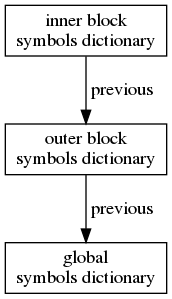
\includegraphics[scale=.35]{blockscopesymboltable.png}
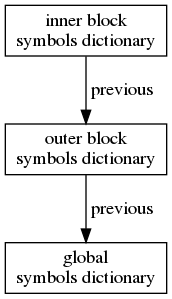
\includegraphics{blockscopesymboltable.png}
\end{figure}

\section{Function Scoping}

The approach in the previous section wears out when we arrive at
functions. A function block should still be able to see global variables.
But, if we call it from within a block, it should not
see the variables in scope for the caller. This is doubly true if the
function calls a function. They should have separate scopes, both
of which can see the global symbols, but not the one belonging to
the other function invocations. To understand the problem, think of
a recursive function. Each invocation needs separate symbols, which
will necessarily have the same names.

To fix this, we need minor changes to the SymbolTable class. First,
we need to add a reference to the caller, which will store the
table in scope at the point of function invocation. Then, we
need new methods to add and discard function scopes.

The only changes to existing code are these

{\footnotesize
\begin{verbatim}
    class SymbolTable:
        def __init__(self, previous, caller):
            self.symbols = {}
            self.previous = previous
            self.caller = caller

        def addInnerScope(self):
            return SymbolTable(self, None)
\end{verbatim}
}

The constructor receives and stores the caller reference. In
addInnerScope we need to pass that parameter, but None works for
regular scopes which have no caller.

There are two new methods for function scope management.

{\footnotesize
\begin{verbatim}
        def addFunctionScope(self, globalTable):
            return SymbolTable(globalTable, self)

        def discardFunctionScope(self):
            return self.caller
\end{verbatim}
}

We make a new scope by constructing with the global table
as previous and the current scope as the caller. Discarding just
returns the caller reference to put the original scope back. Nothing
else changes.

Note that the visitor will need to call these methods correctly and
store their return values.

To see what the symbol table structure looks like with these changes,
consider this example program:

{\footnotesize
\begin{verbatim}
    fun callAdd(a) {
        if (a > 2) {
            return 3 * a
        }
    }

    if (x > 4) {
        while (x > 4) {
            total = callAdd(x)
            x = x - 1
        }
    }
\end{verbatim}
}

Then the full set of symbol tables inside the if in callAdd looks like
this:

\begin{figure}
\centering
%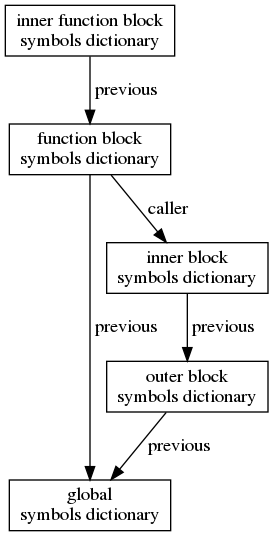
\includegraphics[scale=.35]{functionscopesymboltable.png}
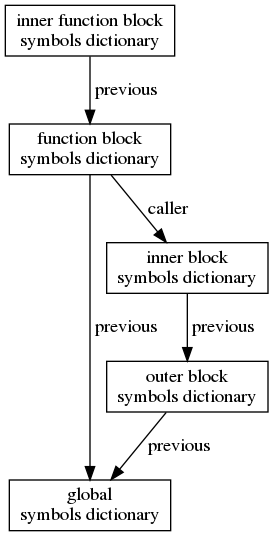
\includegraphics{functionscopesymboltable.png}
\end{figure}

\section{Exercises}

\subsection{Visitor Implemenation}

Create the SymbolTable class and use it to create block scopes
in your existing visitIf and visitWhile methods (in Visitor). You
may need to adjust tests to define variables before scopes begin.

\subsection{Debugging}

Add a debugging method to the SymbolTable class which draws the
structure.
Call the method at strategic points to see the structure grow and
shrink as scopes are added and removed.
Hint: we really have is almost a binary tree now with previous
as the left pointer and caller as the right pointer. There are not
cycles in this graph, but many roads lead to the global table.

\subsection{Testing}

Add a TestSymbolTable class to test the behaviors of the SymbolTable class.

\chapter{Functions}

Functions take input parameters and return values. In some languages
these are called methods, usually because they receive an implicit
object as a parameter. Other languages have similar constructs called
procedures (which don't return values).

Functions are important. They allow us to factor out bits of code
to make things easier to read and to test. They also make code
available to be re-used.

Let's make the overtime pay calculation from the flow of control
chapter into a function. Then it might look something like this:

{\footnotesize
\begin{verbatim}
    function calcpay(hrs, rate) {
        pay = 0
        if (hrs < 40) {
            pay = hrs * rate
        }
        else {
            pay = 40 * rate + (hrs - 40) * rate * 3 / 2
        }
        return pay
    }

    paybob = calcpay(43, 10)
    print paybob

    payjan = calcpay(41, 12)
    print payjan
\end{verbatim}
}

There are quite a few pieces to this function scheme. First, there
is a function definition including the function keyword, the function's
name, a parameter list, and a block.

Inside the block the parameters are visible in a scoped symbol
table that cannot be accessed outside of the function. For instance
pay is not defined unless we are in the function block.

There is a new return statement only valid in the block of a function.

Finally, there is a way to call the function. Here we give its name
and put arguments for its formal parameters inside parentheses.

All of this would be even more complicated if our language supported
types.

\section{Grammar Additions}

We have two new statement alternatives.

{\footnotesize
\begin{verbatim}
    statement : ...
              | 'function' ID '(' paramList? ')' block  # functionDefinition
              | 'return' expr NEWLINE                   # return
              ...
\end{verbatim}
}

The paramList needs a rule. It's already optional, so we need two
choices.

{\footnotesize
\begin{verbatim}
    paramList : ID ',' paramList
              | ID
              ;
\end{verbatim}
}

The lexemes for these ID tokens will only be available inside the function.

Finally, we need a call expression.

{\footnotesize
\begin{verbatim}
    expr : ...
         | ID '(' exprList? ')'         # call
\end{verbatim}
}

An expression list is like a parameter list, but parameters define
names and expressions provide values.

{\footnotesize
\begin{verbatim}
    exprList : expr ',' exprList
             | expr
             ;
\end{verbatim}
}

\section{New Nodes}

We have two new statement productions: functionDefinition and return.
These need nodes. So does the call expr.

\subsection{ReturnNode}

Since return needs to affect the flow of control, we need a new scheme.
If we had statements with addresses in the memory of an assembly program,
we would record the address of the call. Then return would consume that,
and set the program pointer to that spot. The main driver would then
advance to the next statement as if the call was something simpler.

Our scheme is a bit more vexing. One solution is to throw an exception.
Then whoever invoked the act method on the function block would have
to catch that. We could either put the return value in the exception,
or place it into a special spot in the caller's symbol table. I chose
the latter.

It isn't always catch a named (aka checked) Java exception.
But, it always a good idea to use a name when throwing.

{\footnotesize
\begin{verbatim}
    public class ReturnEncounteredException extends RuntimeException {}
\end{verbatim}
}

That lets us end a block immediately upon seeing a return statement.
The caller must then retrieve the return value and reset the symbol tables.

{\footnotesize
\begin{verbatim}
    public class ReturnNode extends Node {
        // the name of the return symbol is chosen to be an illegal identifier
        public static final String RETURN_SYMBOL = "1_return_symbol";
        Node valueNode;
        EvalVisitor visitor;
    
        public ReturnNode(Node valueNode, EvalVisitor visitor) {
            this.valueNode = valueNode;
            this.visitor = visitor;
        }
    
        @Override
        public void act() {
            Integer intValue = getIntValue();
            visitor.set(RETURN_SYMBOL, intValue);
            throw new ReturnEncounteredException();
        }
    
        @Override
        public Integer getIntValue() {
            return valueNode.getIntValue();
        }
    
        @Override
        public boolean getBooleanValue() {
            return getIntValue() != 0;
        }
    }
\end{verbatim}
}

This is very similar to AssignNode. The differences are that it puts
its value into an illegal spot in the symbol table and then throws.

\subsection{FunctionNode}

Some languages allow named parameters, but our functions use
positional parameters instead. The key fact a FunctionNode
to keep track of the list of parameters names in order. It also
needs a block of statements to run.

{\footnotesize
\begin{verbatim}
    import java.util.HashMap;
    import java.util.List;
    import java.util.Map;
    
    public class FunctionNode extends Node {
        List<String> params;
        Node block;
    
        public FunctionNode(List<String> params, Node block) {
            this.params = params;
            this.block = block;
        }
    
        public List<String> getParams() {
            return params;
        }
    
        @Override
        public void act() { }
    
        public void invoke() {
            block.act();
        }
    
        @Override
        public Integer getIntValue() {
            return 0;
        }
    
        @Override
        public boolean getBooleanValue() {
            return getIntValue() != 0;
        }
    }
\end{verbatim}
}

The only methods actually used are the constructor, getParams, and
invoke. FunctionNodes are not put into the program tree, rather
they are kept in a special function symbol table where call statements
can find them.

Remember that the block must include a return statement, otherwise the
call expression will be null. There should be checks for this
somewhere in the compiler.

\subsection{CallNode}

It falls to the call node to direct the execution of the functions.
You don't have to divide things this way. But, I like having only
one complicated node out of these three. I chose CallNode to collect
the complexity.

{\footnotesize
\begin{verbatim}
    import java.util.ArrayList;
    import java.util.List;
    import java.util.Map;
    
    public class CallNode extends Node {
        String functionName;
        List<Node> argNodes;
        EvalVisitor interpretter;
    
        public CallNode(String functionName, List<Node> argNodes, EvalVisitor interpretter) {
            this.functionName = functionName;
            this.argNodes = argNodes;
            this.interpretter = interpretter;
        }
    
        @Override
        public void act() {}
    
        @Override
        public Integer getIntValue() {
            Map<String, Integer> callFrame = interpretter.addCallStackFrame();
            FunctionNode function = interpretter.resolveFunction(functionName);
            List<String> paramNames = function.getParams();
            List<Integer> args = collectArgs();
    
            for (int i = 0; i < paramNames.size(); i++ ) {
                interpretter.set(paramNames.get(i), args.get(i));
            }
    
            Integer answer = null;
            try {
                function.invoke();
            }
            catch (ReturnEncounteredException e) {
                answer = interpretter.resolve(ReturnNode.RETURN_SYMBOL);
            }
    
            interpretter.discardCallStackFrame();
    
            return answer;
        }
    
        private List<Integer> collectArgs() {
            List<Integer> answer = new ArrayList<>();
    
            for (Node argNode : argNodes) {
                answer.add(argNode.getIntValue());
            }
    
            return answer;
        }
    
        @Override
        public boolean getBooleanValue() {
            return getIntValue() != 0;
        }
    }
\end{verbatim}
}

The EvalVisitor will need to collect the parameters for the function node
and the expressions that will fill those in during act in the call node.

The CallNode constructor receives the name of the function, the
list of expression nodes passed into its parameters, and the EvalVisitor
so it can work the call stack.

Before we had functions we needed only one symbol table for our integer
variables. Now we have two extra things. First, a whole new
table for functions. Second a stack of variable symbol tables.

We see this right at the beginning of getIntValue in CallNode. It
starts by asking the interpretter to make a new call stack frame.
That frame will be visible only in the function's block. By using
a stack, it can then unwind that frame when the function exits.
This allows nested function calls, and even recursion.
The stack frame is discarded rigth before returning the answer.

In between, we must retrieve the function from the function
symbol table by calling resolveFunction, a new method in EvalVisitor.
Then we need to pass the values for the parameters.

First, ask the function node for the list of parameter names.
Then call collectArgs to evaluate all the expressions we are
going to pass. Loop through both lists together telling the
interpretter to store the arg value in the current symbol table 
under the name of the parameter.

There are lots of error checks missing here. What if the two
lists are different lengths. We should complain as early as
possible, preferably during compilation or before run time.
As a last resort -- which our little language would probably
need -- right before the function is invoked at run time.
That might require a semantic analysis pass over the Node tree
before calling act on its root.

Once the arguments are safely in the symbol table, it remains
to invoke the function. I chose to add a speical method called
invoke to FunctionNode for this purpose. This makes it clearer
that only call can run the function. Calls to act have no effect.

Finally, the return statement in the block will throw an exception
with a rather long name (ReturnEncounteredException) to break
the block loop. While it does that it puts the integer value of
its expression into the \verb+RETURN_SYMBOL+ slot in the symbol table.
That constant has a name which is invalid as an identifier
so programmers cannot bump into it by accident.

The answer is delivered from that special location by a regular
call to resolve, like any variable lookup.

Those are the nodes. We do need changes to EvalVisitor to build
them and to support the extra symbol table work.

\section{Symbol Tables Have Hatched Out}

In the EvalVisitor, we need to expand out notions of symbol tables.
We need a new regular table for functions. But, we also need a stack
of symbol tables to support privately scoped symbols used in function
bodies.

{\footnotesize
\begin{verbatim}
    Stack<Map<String, Integer>> symbolStack;
    Map<String, FunctionNode> functionTable;
\end{verbatim}
}

Because of the increased complexity, I introduced an explicit
constructor.

{\footnotesize
\begin{verbatim}
    public EvalVisitor() {
        symbolStack = new Stack<>();
        Map<String, Integer> symbolTable = new HashMap<>();
        symbolStack.push(symbolTable);
        functionTable = new HashMap<>();
    }
\end{verbatim}
}

The global symbol table no longer has a name. It is now just the
base element of the symbolStack. This means that resolve and set
need adjustments. They must now peek at the stack to find their table.

{\footnotesize
\begin{verbatim}
    public Integer resolve(String symbol) {
        return symbolStack.peek().get(symbol);
    }

    public void set(String symbol, Integer newValue) {
        symbolStack.peek().put(symbol, newValue);
    }
\end{verbatim}
}

Callers need not know how deep the stack is, nor even that there is
a stack. Calling resolve or set will just work on the top table.

For debugging I added a method.

{\footnotesize
\begin{verbatim}
    public void dumpSymbols() {
        System.err.println( "symbols:\n" + symbolStack);
    }
\end{verbatim}
}

We can call this whenever we are confused about the symbols in scope.
Do note that there is no provision for retrieving global variables
while in a function with this code.

There are methods to insert and remove tables from the stack.

{\footnotesize
\begin{verbatim}
    public Map<String, Integer> addCallStackFrame() {
        Map<String, Integer> newTable = new HashMap<>();

        symbolStack.push(newTable);

        return newTable;
    }

    public void discardCallStackFrame() {
        symbolStack.pop();
    }
\end{verbatim}
}

Finally, there are helpers for the function symbol table.

{\footnotesize
\begin{verbatim}
    public FunctionNode resolveFunction(String name) {
        return functionTable.get(name);
    }

    public void setFunction(String name, FunctionNode node) {
        functionTable.put(name, node);
    }
\end{verbatim}
}

\section{Visiting to Create Nodes}

The last thing I will show is actually the first thing that happens.
As we originally visit the antlr parse tree, we need to visit our
new productions and make their nodes.

\subsection{FunctionNode}

{\footnotesize
\begin{verbatim}
    @Override
    public Node visitFunctionDefinition(ExprParser.FunctionDefinitionContext ctx) {
        List<String> parameters = collectParameters(ctx.paramList());
        Node body = visit(ctx.block());

        String functionName = ctx.ID().getText();
        setFunction(functionName, new FunctionNode(parameters, body));

        return null;
    }
\end{verbatim}
}

To make a function node, we need the parameter names in order and the
block. To put it into the function symbol table, we need its name.
The new setFunction method places it into the table for a CallNode
to find at run time. The only trick is to collect the parameter names.

{\footnotesize
\begin{verbatim}
    private List<String> collectParameters(ExprParser.ParamListContext ctx) {
        List<String> answer = new ArrayList<>();

        while (ctx != null) {
            answer.add(ctx.ID().getText());
            ctx = ctx.paramList();
        }

        return answer;
    }
\end{verbatim}
}

You could write the loop as a C-style three part for loop. But it would
be hard to fit it on one line of reasonable length, so I went with while.
You do need to remember to advance the context along to the next
parameterList at the end of each iteration. I orginally failed to do
that and landed in an infinite loop.

\subsection{ReturnNode}

{\footnotesize
\begin{verbatim}
    @Override
    public Node visitReturn(ExprParser.ReturnContext ctx) {
        return new ReturnNode(visit(ctx.expr()), this);
    }
\end{verbatim}
}

There is almost nothing to a return node, it only needs to visit
its expr child to collect the node which will build the value.
It does need the interpretter in order to place the answer into
the symbol table atop the stack.

\subsection{CallNode}

{\footnotesize
\begin{verbatim}
    @Override
    public Node visitCall(ExprParser.CallContext ctx) {
        String functionName = ctx.ID().getText();
        List<Node> args = collectCallArgs(ctx.exprList());

        return new CallNode(functionName, args, this);
    }

    private List<Node> collectCallArgs(ExprParser.ExprListContext ctx) {
        List<Node> answer = new ArrayList<>();
        while (ctx != null) {
            Node arg = visit(ctx.expr());
            answer.add(arg);
            ctx = ctx.exprList();
        }
        return answer;
    }
\end{verbatim}
}

Collecting the call node is similar to collecting the function node.
It needs a similar helper method to build the list of expression nodes
that will provide the values to the function's parameters. It
returns the newly constructed node like most other statements.

Exercises

1. Add checks to make sure calls provide the correct number of arguments
   to the functions they invoke. Try first with a run time check in
   getIntValue. But, also think about a pass over the tree to check
   for that before the call to act on the root ProgramNode.

2. Turn the symbol table Maps into a separate object. Give those a parent
   attribute. In resolve, walk up the stack looking for symbols that
   are not found in the table at the top of the stack.


\part{Interal Representation}


\chapter{Internal Representation}

To this point, we have used the awesome AST built for us by ANTLR.
While it is amazing how far we have gotten with it, there are limits.
We need to build our own internal representation, if we want to
emit assembly. In other words, to complete the back half of the
compiler we need a new IR.

We will again start with a minimal approach to introduce the concepts.
The internal representation will be a graph of nodes. Ours will
be a tree.\footnote{Some optimization schemes compress this into
a directed graph when two subtrees are identical.}

Each node in this tree will need to be an object descended from the same type.
Traditionally, they would all share the same attributes. But, since
we have objects instead of more primative structures, we don't need to
overload like we would in C.

Each node type will need a constructor for the visitor to call.
They will also need a common method that does something useful.
Our goal is one which emits a target language. But, it could also
draw something useful for debugging, etc. It could even run the
program as we have been doing. In fact, I will start with two
methods in each node: getIntValue (for primitives like
numbers) and act (to interpret like we have been doing). Later,
I will add an emit method to generate assembly output.

Once we have a tree of these nodes, we could implement other tools.
We could write a set of analyzers which walk the tree to enforce
language rules, like missing declarations. When we interpret, those
are run time errors. With an analyzer they can be part of
compilation. This reports the error earlier, before part
of the code runs. Analyzers are beyond our scope. We will generate
errors like this when we notice them as we emit assembly.

Optimizers walk the tree to build an optimized replacement. Since
they are making the same structure, just with different specific
nodes, optimizers can be mixed and matched with each other and
with analyzers. Again, optimizing is an advanced topic beyond our scope.

To distinguish this new tree from the AST built during parsing,
we call this a decorated tree or an internal representation (IR).

\section{Nodes}

Our Node class is quite simple.

{\footnotesize
\begin{verbatim}
    class Node:

        def act(self):
            pass

        def getIntValue(self):
            pass
\end{verbatim}
}

These are the methods each node could implement: act and getIntValue.
The methods implemented with pass statements in the Node parent class
will work for the children that don't need one of the methods.

To start consider the simplest program in our language:

{\footnotesize
\begin{verbatim}
    4
\end{verbatim}
}

When we interpret, this prints `4'.
When this parses, the AST will look like this:

{\footnotesize
\begin{verbatim}
    program
       |
     print
       |
     number
       |
       4
\end{verbatim}
}

This needs the first three node types: ProgramNode, PrintNode, and NumberNode.
I'll show them in reverse order, because they rise in complexity in that
order.

\subsection{NumberNode}

{\footnotesize
\begin{verbatim}
    from Node import Node
    class NumberNode(Node):
        def __init__(self, value):
            self.value = value

        def getIntValue(self):
            return self.value
\end{verbatim}
}

This is a leaf node. It only needs to implement getIntValue.
Its parent will take care of act (and emit when we add it).
All this node needs to do it keep track of the value of its
number and return it upon request.

\subsection{PrintNode}

{\footnotesize
\begin{verbatim}
    from Node import Node
  
    class PrintNode(Node):
        def __init__(self, valueNode):
            self.valueNode = valueNode

        def act(self):
            print(self.getIntValue())
            return self.getIntValue()

        def getIntValue(self):
            return self.valueNode.getIntValue()
\end{verbatim}
}

The statement production for a bare expression will become a PrintNode.
This needs to store the child node during construction. If asked
for the int value, it delegate to that child. Similiarly, to act
during interpretation it looks up the value, prints it to stanard output,
and returns it.

\subsection{ProgramNode}

Finally, the most complicated of our nodes so far will keep a list
of statements and run them in order when asked to act.

{\footnotesize
\begin{verbatim}
    from Node import Node
  
    class ProgramNode(Node):
        def __init__(self, statements):
            self.statements = statements

        def act(self):
            for statement in self.statements:
                statement.act()

        def getIntValue(self):
            return 0;
\end{verbatim}
}

Note that the whole program does not have a useful value to deliver.
We hope no one calls getIntValue on this. If they do, they just get
a zero.

To act on the statements, we just loop through them once in order
asking each of them to act.

\section{Making an IR}

Previously our visitor interpreted the program. Now we will instead
build a tree of Node objects. If the caller wants to interpret the
program, they will call act. Later, they could instead could call emit
to produce assembly.

{\footnotesize
\begin{verbatim}
    from CalcVisitor import CalcVisitor
    from CalcParser import CalcParser
    from ProgramNode import ProgramNode
    from PrintNode import PrintNode
    from NumberNode import NumberNode

    class NodeVisitor(CalcVisitor):
        def visitProgram(self, ctx:CalcParser.ProgramContext):
            statements = []
            rawStatements = ctx.statement()
            for rawStatement in rawStatements:
                statementNode = self.visit(rawStatement)
                if statementNode is not None:
                    statements.append(statementNode)
            return ProgramNode(statements)

        def visitPrint(self, ctx:CalcParser.PrintContext):
            value = self.visit(ctx.expression())
            return PrintNode(value)

        def visitNumber(self, ctx:CalcParser.NumberContext):
            value = int(ctx.NUMBER().getText())
            return NumberNode(value)
\end{verbatim}
}

It is easier to begin reading at the bottom. The visitNumber method
begins in the same way as the interpreting version, by looking up
the text the parser found.\footnote{Remember that there is no reason
to guard against conversion errors here, since the parser would
only bring us here if it found a valid number.}

Then, instead of returning that directly, we make a new
NumberNode with that as its value.

The parent of this number in our simple program is a print statement.
The visitPrint method finds its value by visiting the expresssion, as
it did while interpreting. But, now two things are different. First,
the result of calling visit on the child expression is a Node of some
kind. Second, we need to make a PrintNode to house that child Node.

The tree walk is really directed in visitProgram. That asks for
the raw statements found by the parser and loops over them.
For each one, it calls visit receiving whatever Node type that
produces. If the statement makes no node (think blank lines)
it does not store the result.\footnote{If you are going to emit
the original source code, you have to capture those too.}
If the Node is not None, it goes into the list of statements
which are given to the ProgramNode constructor.

Note again that calling this visitor only returns the ProgramNode
which contains its list of child statements. The caller needs
to call act to gain the original behavior or emit to produce assembly.

\section{Testing the IR}

In software we often hear the terms white box and black testing.
Where that latter certainly implies that we cannot see inside whatever
we are testing. My problem with these as opposites is that white
boxes are also opaque. I prefer to use the terms transparnet and opaque
testing. In this case, we will use transparent testing. This means
that the test will use intimate knowledge of the code being tested.

Here is the new test module to transparently test the NodeVisitor
presented in the prior section.

{\footnotesize
\begin{verbatim}
    from antlr4 import *
    from CalcLexer import CalcLexer
    from CalcParser import CalcParser
    from NodeVisitor import NodeVisitor
    import unittest

    class TestNodeVisitor(unittest.TestCase):
        def test_number(self):
            program = "4\n"
            tree = self.get_tree(program)
            visitor = NodeVisitor()
            answer = visitor.visit(tree)
            self.assertEqual(1, len(answer.statements))
            print_statement = answer.statements[0]
            self.assertEqual(4, print_statement.getIntValue())

    def get_tree(self, program):
        input_stream = InputStream(program)
        lexer = CalcLexer(input_stream)
        stream = CommonTokenStream(lexer)
        parser = CalcParser(stream)
        tree = parser.program()
        return tree

if __name__ == '__main__':
    unittest.main()
\end{verbatim}
}

The \verb+get_tree+ method is the same as in our prior tests. It takes
us through the parsing step which builds the AST.

The \verb+test_number+ method call \verb+get_tree+ to obtain the AST
as before. Then it visits the tree. In earlier tests we could then
examine the result directly for numeric answers. Here we receive
a ProgramNode. First, I decided to check that it contains the correct
number of statements, one in this case. Then I peeked inside
the ProgramNode to retrieve the PrintNode and tested its value
which should be four. This is transparent testing, because I have
used node's internal methods at will. This is a typical approach
for a unit test.

\section{Completing the IR}

We now have a working and tested IR for a subset of our language.
To return to the interpreter we had before, we need to implement
a lot more visit methods. Most of those will need to construct
Node objects.\footnote{Some don't need to do that, like parentheses.
Again, if you needed to regenerate the original program you would
need a node for those too. But for assembly emitting or interpreting
you don't.}

%\chapter{Types}

So far our language has only worked with integers. This is
an obvious problem. It would be more useful if it worked
exclusively with floating point numbers. That would still
leave it limited. It is time to talk about types.

We actually introduced a parallel type for functions in
the last chapter. Anything with a name resolved at runtime
should be part of a single type system. Leaving functions separate
seemed to make our lives easier. Now we will incorporate
them into the type system along with ints and floats.

We couldn't expand the scheme of making a separate symbol
for floating point numbers, like we initially did for functions.
The problem is that the arithmetic operators
are shared by integer and floating point math. Since
those two must share, we should make a comprehensive
system for all symbols.

Some language introduce new operators to simplify the type
system. Perl has separate comparison operators for strings
and a separate symbol for concatentation, reserving the
plus sign for actual Math. But, addition of numbers still
works with both ints and floats.
If a single operator will work with two disperate kinds
of data, you must make it part of a type system.

\section{Floating Point Numbers}

As a first step we need to define what we mean by a floating
point number. How we will recognize it with a token?
Here are some of the things we want to be floating point numbers:

{\footnotesize
\begin{verbatim}
    1.2
    0.2
    45.
    .15
\end{verbatim}
}

For now, we'll avoid numbers that need exponents. Many languages
include things like 6.02e23. We'll leave that as an exercise.
We could allow negative versions of these as well. But see
the section on Unary Negation in the Odds and Ends chapter
for what we really need to do.

When you have lots of choices you should immeidately think
of the as alternative operator: |. We have used that
extensively in grammars. It works in regular expressions too.
Let me list the pieces along with what they match. Then,
we'll combine them.

\begin{tabular}{l l l}
To Match  & Use                    & In English \\
.15       & '.' [0-9]+             & a dot, then one or more digits \\
0.2       & '0' '.' [0-9]+         & a zero, a dot, and one or more digits \\
14.12     & [1-9][0-9]* '.' [0-9]* & any digit by zero, any number of digits, \\
45.       &                        & a dot, more optional digits \\
\end{tabular}

Putting these together we have a new lexer definition:

{\footnotesize
\begin{verbatim}
    FLOAT: '-'? ( '.' [0-9]+ | '0' '.' [0-9]+ | [1-9][0-9]* '.' [0-9]* )
\end{verbatim}
}

For now, we'll keep the possibiity of the numbers themselves being
negative. (Again, we really need unary negation.) Also, we have
no limits here. At some point during compilation, we need to notice
if a literal number is two big to fit in storage and raise an exception.
We also need to report an error if runtime computations result
in a number that is too big for storage.

Once we have a definition of what will count as a floating point
number, it is trivial to add them to the grammar. It is just another
expression alternative.

{\footnotesize
\begin{verbatim}
    expr : ...
         | FLOAT        # float
\end{verbatim}
}

This adds a visitFloat method to the parse tree walk. We'll need FloatNode
to go with that.

\section{A Simple Type System}

Naively allowing FLOATs as expressions will not work. We need to make
structural changes to the grammar and later to the parse tree walker,
symbol table, and nodes.

First, variables will need a type. This is foundational. When we first
encounter a variable, the programmer must tell us the type. Many languages
allow this type in a bare declaration. Java does this. It invites the
developer to use undefined variables, resulting in an error. Java calls
this a null pointer exception. You could prevent that by requiring
assignment during declaration. I will follow Java's garden path to
see how we need to report those errors later.

In addition to typing variables, we need types in two other places.
First, in the parameters to functions. Second, for the return values
of those functions. Here is the new definition of statement:

{\footnotesize
\begin{verbatim}
    statement : 'print' expr NEWLINE                            # printExpr
              | type ID NEWLINE                                 # declare
              | type ID '=' expr NEWLINE                        # declareAssign
              | ID '=' expr NEWLINE                             # assign
              | 'if' '(' conditional ')' block else?            # ifStatement
              | 'while' '(' conditional ')' block               # whileStatement
              | 'function' ID '(' paramList? ')' ':' type block # functionDefiniton
              | 'return' expr                                   # return
              | NEWLINE                                         # blank
              ;
\end{verbatim}
}

There are two new statement alternatives: one for bare declaration, one for
declaration with assignment. The function alternative has a new ':' type
addition for the return value. You could choose to use the Java approach
instead, by listing the type before the function name.

{\footnotesize
\begin{verbatim}
    type : 'int' | 'float' ;
\end{verbatim}
}

I chose the familar int and float types. They may confuse the Java developer,
because float will be implemented with Double. Since we are implementing in
Java that will simplify everything, since Double is the default float type
there. Unless we wanted to implement our own libraries to do the actual
calculations (or emit careful assembly) there is no use to fighting this.

Note that function does not appear in the type rule. We only allow
proper definitions with parameter lists.

The final alteration to the grammar is in the definition of paramList.
Now that parameters need a type, they need a rule.

{\footnotesize
\begin{verbatim}
    paramList : param ',' paramList
              | param
              ;

    param : type ID ;
\end{verbatim}
}

\section{Symbols}

With symbols that have types, we need a class to describe them. Like Nodes,
each type of symbol will inherit from this abstract class.

{\footnotesize
\begin{verbatim}
    public abstract class Symbol {
        String name;
        SymbolType type;
    
        public Symbol(String name, SymbolType type) {
            this.name = name;
            this.type = type;
        }
    
        public static Symbol getInstance(String typeName, String symbolName) {
            Symbol answer = null;
    
            switch (typeName) {
                case "int" :
                    return new IntSymbol(symbolName);
                case "float" :
                    return new FloatSymbol(symbolName);
                case "function" :
                    return new FunctionSymbol(symbolName);
            }
    
            return answer; // unreachable, the grammar will insist on a valid choice
        }
    
        public abstract Integer getIntValue();
        public abstract Double getFloatValue();
        public abstract FunctionNode getFunctionValue();
        public abstract void setIntValue(Integer newValue);
        public abstract void setFloatValue(Double newValue);
        public abstract void setFunctionValue(FunctionNode functionValue);
    
        public String getName() {
            return name;
        }
    
        public SymbolType getType() {
            return type;
        }
    
        public enum SymbolType {
            INT,
            FLOAT,
            FUNCTION
        }
    }
\end{verbatim}
}

At the bottom is the SymbolType. We make an entry there for
each type. The core facts of all symbols are then a name and a type.
This they share in the common parent class.
There are accessors for those attributes.

The subclass instances will know their values. They have accessors for
those values. If the type cannot meaningfully deliver one of the values,
it will throw an exception. If it has a choice, it should try to respond
with a good value. In particular, when an int is asked for a float
value, it should return its value as a float.

There is a factory here to create instances of the proper type. This
saves the main parse tree visitor from having to do that. There are
other reasonable designs.

The subclasses themselves are really just houses for a value.
Here is the class for ints. The others are similar.

{\footnotesize
\begin{verbatim}
    public class IntSymbol extends Symbol {
        Integer value;
    
        public IntSymbol(String name) {
            super(name, Symbol.SymbolType.INT);
        }
    
        public Integer getIntValue() {
            if (value == null) {
                throw new RuntimeException("Symbol '" + getName() +
                    "' used before definition");
            }
            return value;
        }
    
        public Double getFloatValue() {
            return Double.valueOf(value);
        }
    
        public FunctionNode getFunctionValue() {
            throw new RuntimeException("Symbol '" + getName() +
                "' is an int which cannot return a float");
        }
    
        public void setIntValue(Integer newValue) {
            value = newValue;
        }
    
        public void setFloatValue(Double newValue) {
            throw new RuntimeException("Symbol '" + getName() +
                "' is an int which cannot hold a float");
        }
    
        public void setFunctionValue(FunctionNode illegal) {
            throw new RuntimeException("Symbol '" + getName() +
                "' is an int which cannot hold a function");
        }
    
        public String toString() {
            return "int " + getName() + " " + getIntValue();
        }
    }
\end{verbatim}
}

\section{Symbol Tables}

The Symbol objects will live in a SymbolTable.

{\footnotesize
\begin{verbatim}
    import java.util.HashMap;
    import java.util.Map;
    
    public class SymbolTable {
        Map<String, Symbol> table;
        SymbolTable parent;
    
        public SymbolTable(SymbolTable parent) {
            table = new HashMap<String, Symbol>();
            this.parent = parent;
        }
    
        public static SymbolTable generateGlobalSymbolTable() {
            return new SymbolTable(null);
        }
    
        public SymbolTable getParent() {
            return parent;
        }
    
        public Symbol resolve(String name) {
            if (table.containsKey(name)) {
                return table.get(name);
            }
            else if (parent != null) {
                return parent.resolve(name);
            }
            else {
                throw new RuntimeException("No such symbol " + name);
            }
        }
    
        public void set(String name, Symbol symbol) {
            table.put(name, symbol);
        }
    
        public String toString() {
            StringBuilder sb = new StringBuilder();
            for (SymbolTable l = this; l != null; l = l.parent) {
                sb.append(l.table + "\n");
            }
            return sb.toString();
        }
    }
\end{verbatim}
}

The table itself is a Map, specifically a HashMap. When you construct a new
one, you pass in the parent. This allows us to chain the tables. More on
that in a moment.

For clarity, I created generateGlobalSymbolTable to make a parentless table.
That is for the interpreter to use for the global symbols. Other tables will
be temporary children during function execution.

When you are done with a function's table, the interpeter replaces the
current SymbolTable with its parent. To find that it calls getParent.

Calling resolve hands you the Symbol in the table. If it isn't there, the
parent is searched recursively. Only if the name is in none of the current
tables does the caller receive an exception. This is chaining, which allows
us to use global variables in functions. But, local variables in the block
of the function and its parameters will hide globals.

Java doesn't have globals in this sense. Yet, the same idea applies in instance
methods which use class attributes.

Set is simpler, since new variables always go in the top most table. (We
think of these tables as a stack.)

Notice that toString here walks back through the stack of tables so callers
can see everything. This is great for debugging.

\section{Interpreter Symbol Table Management}

In my approach, the interpreter knows all about the symbol tables. It keeps the
root table for globals and facilitates all actions on tables. These are the helpers.

{\footnotesize
\begin{verbatim}
public class EvalVisitor extends ExprBaseVisitor<Node> {
    SymbolTable symbols = SymbolTable.generateGlobalSymbolTable();

    public Symbol declare(String type, String id) {
        Symbol newSymbol = Symbol.getInstance(type, id);
        symbols.set(id, newSymbol);
        return newSymbol;
    }

    public Symbol resolve(String name) {
        return symbols.resolve(name);
    }

    public void setValue(String name, Integer newValue) {
        symbols.resolve(name).setIntValue(newValue);
    }

    public void setValue(String name, Double newValue) {
        symbols.resolve(name).setFloatValue(newValue);
    }

    public void setReturnValue(String name, Symbol symbol) {
        symbols.set(name, symbol);
    }

    public void pushCallStackFrame() {
        symbols = new SymbolTable(symbols);
    }

    public void popCallStackFrame() {
        symbols = symbols.getParent();
    }

    public void dumpSymbolTables() {
        System.err.println( "Symbols:\n" + symbols.toString());
    }
\end{verbatim}
}

The symbols variable always points to the top of the symbol table stack.
It starts with the parentless root for globals during class initialization.
Declaring a symbol uses the type name from the grammar: int, float, function
and the name. Even if the programmer is assigning during declaration, we
do that in two steps: declare then assign.

Resolve delivers the Symbol of the given name to the caller, or throws an
error if that symbol table is not in the current stack. Note that it is
up to the caller to notice if the the type of the symbol is illegal.
We could have a compilation pass between EvalVisit's walk and calling
act on the root program node.

The setValue methods allow the caller to provide the properly typed value
for the symbol. Mismatches ought to be checked somewhere.

The return statement has a special purpose helper so that it doesn't need
to declare the return variable. It always has the same name and it
could call declare and set like everyone else. But, this syntactic sugar
looked good to me.

To start a function call, CallNode will ask the interpreter to pushCallStackFrame.
This creates a new table, whose parent is the current one. It becomes the
current one. That parent link in the SymbolTable class is what makes it
capable of being a stack. This method affects the push.

When the CallNode is done with the function invocation, it must retrieve
the return value from the current symbol table, then discard that by
calling popCallStackFrame. That prevents symbols from bleeding
between function calls.

Finally, a nice way to call toString on the top symbol table is available
for anyone who has an interpreter instance handy: dumpSymbolTables.

\section{Visiting Methods and Nodes}

We need some visit method adjustments for the statements we introduced:
visitDeclare and visitDeclareAssign are brand new. We also need to adjust
visitFunctionDefinition due to the increased complexity in gathering the
parameters.

We also need to visitFloat, which is a lot like visitInt.

The CallNode needs changes to account for typed parameters.

\subsection{Visiting Methods}

Bare declarations are compile only. You don't need to store for those.

{\footnotesize
\begin{verbatim}
    @Override
    public Node visitDeclare(ExprParser.DeclareContext ctx) {
        String type = ctx.type().getText();
        String id = ctx.ID().getText();

        declare(type, id);
        return null;
    }
\end{verbatim}
}

We lookup the type and the id, then use the declare helper. There
is a bug here. Either we need to require values when variables
are declared in a function's block, or we need a way to note the
declaration so it can be added to the function's symbol table.

For declarations providing initial values, we do something similar,
but return an AssignNode.

{\footnotesize
\begin{verbatim}
    @Override
    public Node visitDeclareAssign(ExprParser.DeclareAssignContext ctx) {
        String type = ctx.type().getText();
        String id = ctx.ID().getText();
        Node valueNode = visit(ctx.expr());

        declare(type, id);
        return new AssignNode(id, valueNode, this);
    }
\end{verbatim}
}

Defining functions is also a compile time activity. We don't want them
in the runtime tree lest they run by accident. There several changes
to visitFunctionDefinition.

{\footnotesize
\begin{verbatim}
    @Override
    public Node visitFunctionDefiniton(ExprParser.FunctionDefinitonContext ctx) {
        List<Parameter> parameters = collectParameters(ctx.paramList());
        Node block = visit(ctx.block());
        String returnType = ctx.type().getText();

        FunctionNode functionNode = new FunctionNode(parameters, returnType, block);

        String functionName = ctx.ID().getText();
        declare("function", functionName);
        Symbol functionSymbol = resolve(functionName);
        // we need to put the node into the symbol table, not just record its name
        functionSymbol.setFunctionValue(functionNode);

        return null;
    }
\end{verbatim}
}

The collection of parameters is only cosmetically different here. The list is of
type Parameter instead of String. There is more work in collectParameters as we
will see below.

Collecting the block is the same. Now there is a return type too. These are
passed to the FunctionNode constructor. We again lookup the function's name,
but now we put it in the main symbol table with the variables. First, we must
declare it. Then we give a value by resolving the name to retrieve the
function's symbol and storing the node there.

\subsection{CallNode Changes}

Now that there are two types, callers could be expecting an int or a float
to come back from a function. As with other cases, we are happy to deliver
an int as a float, but using a float as an int is an error.

{\footnotesize
\begin{verbatim}
    import java.util.List;
    
    public class CallNode extends Node {
        String functionName;
        List<Node> arguments;
        EvalVisitor interpretter;
    
        public CallNode(String functionName, List<Node> arguments, EvalVisitor interpretter) {
            this.functionName = functionName;
            this.arguments = arguments;
            this.interpretter = interpretter;
        }
    
        @Override
        public void act() { }
    
        private Symbol callFunction() {
            FunctionNode function = getFunctionNode();
            interpretter.pushCallStackFrame();
    
            passParameters(function);
    
            try {
                function.invoke();
            }
            catch (ReturnEncounteredException e) {
                // expected, happens whenever the function hits a return statement
            }
    
            Symbol returnValue = interpretter.resolve(ReturnNode.RETURN_SYMBOL);
    
            interpretter.popCallStackFrame();
    
            return returnValue;
        }
    
        private FunctionNode getFunctionNode() {
            Symbol functionSymbol = interpretter.resolve(functionName);
            return functionSymbol.getFunctionValue();
        }
    
        private void passParameters(FunctionNode function) {
            List<Parameter> parameters = function.getParameters();
    
            // TODO verification of count match (correct number of args)
            for (int i = 0; i < parameters.size(); i++) {
                Parameter parameter = parameters.get(i);
                Node valueNode = arguments.get(i);
    
                // verify that the type on the parameter can be delivered by the valueNode
                if ("int".equals(parameter.getTypeName())) {
                    if (! valueNode.canBeInt()) {
                        throw new RuntimeException("parameter " + parameter.getName() + " to function " +
                                functionName + " must be int");
                    }
    
                    interpretter.declare("int", parameter.getName());
                    interpretter.setValue(parameter.getName(), valueNode.getIntValue());
                }
                else {
                    interpretter.declare("float", parameter.getName());
                    interpretter.setValue(parameter.getName(), valueNode.getFloatValue());
                }
            }
        }
    
        @Override
        public boolean canBeInt() {
            FunctionNode function = getFunctionNode();
            return function.canBeInt();
        }
    
        @Override
        public Integer getIntValue() {
            if (!canBeInt()) {
                throw new RuntimeException("Float function " + functionName + " asked to give an int");
            }
    
            Symbol returnValue = callFunction();
            return returnValue.getIntValue();
        }
    
        @Override
        public Double getFloatValue() {
            Symbol returnValue = callFunction();
            return returnValue.getFloatValue();
        }
    
        @Override
        public boolean getBooleanValue() {
            return false;
        }
    
        public String toString() {
            return "call " + functionName + "(" + arguments + ")";
        }
    }
\end{verbatim}
}

The attibutes, constructor and act methods are unchanged. That latter still does nothing.
Both getIntValue and getFloatValue work similarly. The only difference in structure
is that getIntValue complains if the function cannot return an int.
Both invoke callFunction to get the Symbol from the return statement in the function block.
Then they return the value from it.

It uses the getFunctionNode method to ask for symbol table lookup on the name of the function,
which it returns as the FunctionNode from that. Error checking is in order here.
Then, it asks the interpreter to add a symbol table to the stack. I called this
pushCallStackFrame because other languages will have other things to include
besides the symbol table. In particular if you are aiming for assembly, you
are going to need to include the return address so the program can keep running
from where it left off.

Once the new symbol table is in place, I need to passParameters into it.
I do that by walking two lists at once: the function's parameters and the
call's arguments. The types are compared and the usual complaint is raised
when a programmer asks to stuff a float value into an int slot.
The rest is just like variable declarations from assign statments.

With the parameters in place, it is time to invoke the function. We are expecting
the ReturnEncounteredException. The exception itself carries no information,
but it gives us back control at this point. Traditionally, statements would
be in sequential memory locations (for assembly). Then the return statement
would look in the top frame on the call stack for the line number to jump to.

The return statment puts the return value into the symbol table in a location
with an illegal name, to avoid colliding with programmer code. That symbol
name is \verb+ReturnNode.RETURN_SYMBOL+. Once we are holding that, it is time
to pop the symbol table off the stack and give back the value.

Exercises

1. Expand the alternatives in the regular expression for FLOAT to
   allow exponents. A lot of languages use the same notation.
   Visit https://www.json.org to see all the options. Keep in mind
   that in JSON number includes integers. Avoid those cases.

2. Fix the bug that puts variables declared without values in function blocks
   in the global symbol table. Either, tell the function node about
   the declaration so it can be put in the right table at run time,
   or call an error demanding that these declarations receive initial
   values.

3. Add a validation to ensure that a function has a return statement.

4. Add a void return type so functions can act as procedures. They
    would then only be useful for side effects, possibly printing.

5. Add better error messaging if the programmer attempts to call an
    undefined function.

%\include{constantFolding}

\part{Emitting Assembly}

\chapter{Pseudo-Assembly Language}

The first time I worked through the Dragon book I wanted to get
all the way to assembly. The problem was that I was working on this
self study at work (where I was there to answer phones that rarely
rang) and at home. These environments had different computer architecture.
Thus, the assembly was different. My solution was to write my own
assembly language. I called it the pseudo-assembly language (PAL).
It was then written in Perl. I've later implemented it in Java
and more recently replicated it with ANTLR in Java.

There are two advantages to PAL: it is device independent and it is
simpler than a genuine assembly. PAL has only one assembly directive
and nineteen statements. Most assemblies are far more complex.

\section{A Directive and All 19 Commands}

\subsection{Memory}

In a modern assembler there are segments of memory. First comes
the global symbols, then the program data, than a chunk for
the stack and heap. Typically the stack and heap use the same
block of memory and grow toward each other as functions are called
(stack expands) and dynamic variables are created (heap expands).

This is a bit safer than old school assembly where the data area
and code shared space. That allowed you to change the code with
code. That is dangerous for sanity and security.

PAL is old school. You can allocate memory whenever you want, but
you should only do it at the top of the program. But, it has
a separate stack for function calls. Real assembly would have
no where to put that. Implementing in Java gives us access to its heap.

The one assembly directive in PAL is alloc which takes one parameter:
the number of slots to allocate. Each slot holds a floating point
number. To be able to use the memory, you need to label the line.
Every line in PAL can have an optional label which is an identifier
followed by a colon.

{\footnotesize
\begin{verbatim}
    x: alloc 1
\end{verbatim}
}

This creates a labeled location in memory holding one value called x.

\subsection{Convenience}

Since PAL is implemented in a high level language, it is easy enough
to print to the console and receive values from there.
For this there are three commands: prompt (to print text messages),
prt (to print variable values) and take (to receive and store values).

{\footnotesize
\begin{verbatim}
    n: alloc 1
       prompt "Enter an integer ->"
       take n
       prt n
\end{verbatim}
}

This prints the prompt, receives the input, and stores it in the location
labeled n. Then it prints it from n.

That makes three of the nineteen statements.

\subsection{Calculations}

As with traditional assembly, current versions of PAL require that
calculations be done in registers of which there are not many.
For instance, to add numbers we need to first move one into a
register, then add the other one to that register. Finally, we
need to move the value from the register to a named location so
we have the register free for subsequent calculations.

{\footnotesize
\begin{verbatim}
    x: alloc 1
    y: alloc 1
    z: alloc 1

       prompt "Enter x ->"
       take x
       prompt "Enter y ->"
       take y
       move x %regA
       mult y %regA
       move %regA z
       prt z
\end{verbatim}
}

This effects the calculation z = x + y and prints the value in z at the end.

In addition to mult for multiplication, PAL offers add, subt (subtract),
and div (for division).

This is five more statements (subtotal 8).

\subsection{Conditional Logic}

Each conditional operation statement takes two operands to compare
and a third operand which is a label to jump to if the comparison holds.

{\footnotesize
\begin{verbatim}
    hours:      alloc   1

                prompt  "Enter hours worked -> "
                take    hours
                brgt    hours   40.0    overtime
    regular:    prompt  "You only get regular pay"
                jump    finish
    overtime:   prompt  "You deservere overtime"
    finish:     end     0
\end{verbatim}
}

This is a lot of overhead to show one new command. This asks for a value
for hours. Then it tests to see if that value is greater than 40.
If so, it jumps to overtime. If not, it falls through.
When you set up logic like this, you usually need jump to avoid the
blocks you don't want (overtime from regular pay in this case).
The jump command is unconditional, but you should use it to implement
standard logic structures and not to bounce around the program randomly.

The end command stops the program, giving the shell that started it the
value of the operand as a status. That must be an int.

There are six conditional operators

\begin{tabular}{l l}
    Command &   Operator \\
    brgt    &   > \\
    brge    &   >= \\
    brlt    &   < \\
    brle    &   <= \\
    breq    &   == \\
    brne    &   != \\
\end{tabular}

All work the same way. The operator of the command is placed between
the first two operands. If the condition is true, control jumps to
the third operand, otherwise it falls through.

That's six more commands for the conditionals, plus jump and end for
total 8 new commands. (running subtotal 16).

\subsection{Subroutines}

PAL supports only a primative notion of subroutines, notably because
all variables are global. But, it does keep a stack of call locations
to which you can return.

Consider this rather ellaborate example which computes factorial.

{\footnotesize
\begin{verbatim}
    n:         alloc      1
    original:  alloc      1
    answer:    alloc      1

               prompt     "Enter and integer n, I'll find n! ->"
               take       n
               move       n       original
               move       1.0     %regB
               gosub      fact
               move       %regB   answer
               prompt     "Factorial of"
               prt        original
               prompt     "is"
               prt        answer
               end        0
    fact:      brle       n     1.0     base
               mult       n     %regB
               move       n     %regA
               subt       1.0   %regA
               move       %regA n
               shower
               gosub      fact
    base:      ret
\end{verbatim}
}

It starts in similar manner to prior examples. It takes a number from
the user, stores it as original (for use in the final prt command).
It puts the starting number one into register b, where the multiplications
will take place.

Then it uses the gosub command to transfer control to the fact label.
The difference between gosub and jump is that the latter can include
a ret command to go back to the calling location (or actually the
line right after that). As this example demonstrates, you can do
this recursively. But, again, you are stuck with global variables.
This is the mimimum stack frame possible: only the return location is
stored.

Now we have seen the alloc directive and all nineteen of the PAL commands.
% summary table

\section{Accessing Modes and Arrays}

So far we have only seen the commands with named memory locations
holding single values and the registers. To implement arrays (which
you could use to make your own stack for gosubs) we need addressing modes.
These allow us to use one allocated memory location to hold the
address of a different memory location. The allocation looks like
this

{\footnotesize
\begin{verbatim}
    score:  alloc 1
    scores: alloc 5
\end{verbatim}
}

The score here is a pointer which tells us where we are in the array
called scores. Now you know why alloc takes an operand. These arrays
are fixed in size.

To obtain the pointer value at the top of the array, PAL uses the
ampersand.

{\footnotesize
\begin{verbatim}
    move    &scores     score
\end{verbatim}
}

In this memory segment, the first word score is in location zero.
The scores array begins at position one and continues through position
six. So, \verb+&scores+ is one.

{\footnotesize
\begin{verbatim}
    +---------+-----------+
    | address | variable  |
    +---------+-----------+
    |       0 | score     |
    +---------+-----------+
    |       1 | scores[0] |
    +---------+-----------+
    |       2 | scores[1] |
    +---------+-----------+
    |       3 | scores[2] |
    +---------+-----------+
    |       4 | scores[3] |
    +---------+-----------+
    |       5 | scores[4] |
    +---------+-----------+
\end{verbatim}
}

This is why almost all languages index arrays from zero. Then the address
of the first element is the address of the array. All slots are
the address of the zero element plus the width of the memory times the index.
Here the memory width is one. In an acutal assembly, it would be the
width in bytes of each array element.

Once we can store an address, we need a way to indicate that it is
an address that needs to be dereferenced. PAL uses @ for that.
Suppose score is two, to store the third element of the array we
can use

{\footnotesize
\begin{verbatim}
    move 2      score
    take @score
\end{verbatim}
}

Of course, we need to do this in a loop, as we will soon see.

Finally, it is highly useful to be able to increment while we use
the pointer in this way. For that we can add a plus sign after the
expression: @score+. This will first use the current value of the
score pointer, but then increment immediately after. That makes
moving through the elements much easier.

Here is an example that accepts five test scores, finds the maximum
among them and scales all of them by dividing each by the maximum.
This is a rescaling rule I used when I taught Math, in the dark ages
of the prior millenium.

{\footnotesize
\begin{verbatim}
    score:  alloc       1
    max:    alloc       1
    scores: alloc       5
    
            move        &scores     score
            move        0.0         max
            move        0.0         %regA
    input:  brge        %regA       5.0         proc
            prompt      "Enter score"
            take        @score
            add         1.0         %regA
            brlt        @score      max         next
            move        @score      max
    next:   move        score       %regB
            add         1.0         %regB
            move        %regB       score
            jump        input
    
    proc:   move        &scores     score
            move        0.0         %regA
            prompt      "num scaled_score"
    output: brge        %regA       5.0         done
            move        @score+     %regC
            div         max         %regC
            prt         %regA       %regC
            add         1.0         %regA
            jump        output
    
    done:   end         0
\end{verbatim}
}

As in the explanation above, score is the pointer to the current
array value, scores holds the array. These are like the diagram
of the memory. The max slot will hold the high score, which
becomes the divisor for all the scores in the output section.

After allocating memory, move stores the address of the scores array
in score, as we have already seen. Then zero becomes the max, to
have a starting point. I use register A to hold the counter which
goes from zero through four, so that I don't overflow the array.
In an old school assembly overflowing arrays re-wrote other variables
or even the programs instructions. These buffer overrun errors
were the source of all sorts of problems including security breaches.

The scores are collected from the user beginning at input, which
checks to make sure we are under the limit of the array. When we
get to five slots, it moves us to proc (short for process).

While we are still collecting, the user receives an "Enter score"
prompt. Their value is taken and stored in the array slot the score
pointer currently references. Then, register A is incremented.

With the loop managment and actual input handled, the code moves
on to identifying the high score. The brlt comparison checks
whether the value we have just received (@score) is less than
the max previously recorded. If so, this is lower than the max
and we don't need to do anything further with it, so we jump to next.
But, if not, we need move the new value into max.

This bit of logic is why we cannot yet use an incrementing addressing
mode. Instead, beginning at next, the score pointer goes into
register B, where it is incremented. The result is moved back
into score. The result of those three commands is to bump the pointer
forward by one. With pointer incremented, we jump back to the
top of the loop, which will end if we have now exceeded the limit
by reaching five. (Remember our array values are zero through four.)

When the input loop ends, it sends us to proc to process the scores.
There the score pointer is reset to the top of the scores array.
Register A is also reset so that it can again count to keep
us within the array bounds. The user sees text "\verb+num scaled_score+"
which is the heading row of a primitive table.

Having re-initialized the array mechanics, execution flows into
output. That labeled line looks just like input, except for
where it goes when we reach the end of the array. This one goes
to done, to exit the program.

Right below the output labeled line, we see the addressing mode.
The value pointed to by score is moved the register C, and the
score pointer is then post-incremented (in C source code this
might look like: regc = scores[score++]).

The value in register C, which is one of the scores, is divided
by the max we recorded during the first loop. The index and
that division result are printed for the user to see. Then the
loop index is incremented and jump returns us to the top of
the output loop.

Some languages have decrement addressing modes, or even more
exotic ones, like double indirect post auto-increment. PAL sticks
with pre and post increment.

\begin{tabular}{l l }
    Mode                      &  Syntax \\
    address of                &  \verb+&arrayvar+ \\
    value of pointer          &  @pointer \\
    value with post-increment &  @pointer+ \\
    value with pre-increment  &  @+pointer \\
\end{tabular}

Now we have seen PAL in all its glory, which admittedly does not shine
too brightly.
It is small and doesn't have too many features, but you can write a lot
of code in it.

\section{Exercises}

% from the original Intro to Computer Science using Perl
% (A novices guide to writing software)

\subsection{Counting Down}

Write a PAL program to print odd numbers from 9 down to 1.

\subsection{Interest}

Write a PAL program to calculate the final balance in a banking account
which begins with \$500 and earns 5\% per year, compounded monthly.
Modify the program to accept the initial investment, rate of interest,
and years as user input.

\subsection{Debt}

Write a PAL program to estimate how long it will take to pay off
a credit card balance.

\subsection{Successful Semester?}

Compute a semester GPA for a student taking five courses. Have the
user enter the credit hours and grade for each class. Store those
in PAL arrays. Then, compute the grade points for each course
and compute the GPA.

%\include{emittingPAL}
%\include{actualAssembly}
%\include{emittingAssembly}

\appendix
\chapter{Language Exercises}

Even though there are mounds of features our language from the prior
chapters does not have, it actually pretty sophisticated. Many tasks
in computing are done with languages that don't have functions,
loops, or even variables.

The odds that you will use the concepts and tools from the early
part of this book to work on a production compiler are not great.
But, there are lots of problems which come up in the day to day
life of the working developer that benefit from these ways of
thinking.

This chapter presents some exercises you can do to practice grammar
based parsing and AST use.

\section{ASCII Art}

When I took typing in junior high, our teacher gave us fun handouts
(well, she thought they were fun). Each line on the handout was one
line to type. Everything on the line was a number followed by a letter
to type. When you followed instructions, you got ASCII art.

Example Input

3 45-
1
5 5-4 5-4 5-4 5-4 5-
1
3 45-

(Note that the lines that start with ones have a single trailing space.)

Example Output for that input

   ---------------------------------------------

     -----    -----    -----    -----    -----

   ---------------------------------------------

[ we need a way to provide examples here ]

Make a grammar that parses this input and a corresponding visitor
that can emit the output.

\section{Story Board}

I like to use dot from the graphviz project. Part of the reason is
beacause it is text based. That means you can easily generate input
for it.

Consider a little language to diagram a play or screen play.

Example Input

    act {
        scene meetcute "BOY meets GIRL, but he is rude"
        scene ...
    }

Example Output

...

Convert the input into a dot directed graph, which is a story board..
Either install graphviz or use https://sketchviz.com/new to see
your results.

\section{Code Generator}

There are many tools that generate code. Every IDE has a set of
generators. These can save a lot of typing, especially in languages
with a lot of boilerplate. Get in on the generating act yourself.

Example Input

    class Parent {
        int x
        String name
    }

    class Child from Parent {
        String nickname
    }

From this generate classes with proper inheritance. Provide:
    attributes
    a constructor to accept and store those attributes
    accessors for them

Use any language that supports class based inheritance are you target.

\section{Emitting Target Code}

Choose a version of the language we developed in prior chapters.
Emit python for programs in the language. This involves writing a new
visitor which spits out python instead of running the program.
You'll know your solution is working when the python program runs
with the same results as the original (although it will probably chat less).

Use a version of the lanugage which has at least fully functioning
arithmetic. Start with that. Then add variables, flow of control (if
and while), and -- if you dare -- functions.


\backmatter
\addcontentsline{toc}{chapter}{Index}
\printindex
\end{document}
